\section{Principes de base}

\subsection{Rédaction}

\begin{frame}[fragile=singleslide]
  \frametitle{Rédaction}
  \begin{itemize}
  \item On se concentre sur le contenu et la \alert{structure} du
    document, pas sur son \alert{apparence}
      \bigskip
      \begin{tabbing}
        \verb=\textbf{titre}= \qquad\= \faArrowRight \qquad\= \verb|\section{titre}| \\[6pt]
        \verb|\textit{texte}| \> \faArrowRight \> \verb|\emph{texte}|
      \end{tabbing}
      \bigskip
  \item Apparence prise en charge par {\LaTeX} et généralement préférable de ne
    pas la modifier
  \item Mots séparés par une ou plusieurs \alert{espaces}
  \item Paragraphes séparés par une ou plusieurs \alert{lignes blanches}
  \item Utilisation de \alert{commandes} pour indiquer la structure du texte
  \end{itemize}
\end{frame}

\subsection{Structure d'un document}

\begin{frame}[fragile]
  \frametitle{Structure d'un document {\LaTeX}}

  Un fichier source {\LaTeX} est toujours composé de deux parties:

  \hfill
  \begin{minipage}{0.75\linewidth}
\begin{lstlisting}[emph={documentclass,begin,end,document}]
\documentclass[11pt,french]{article}
  \usepackage{babel}
  \usepackage[autolanguage]{numprint}
  \usepackage[utf8]{inputenc}
  \usepackage[T1]{fontenc}

\begin{document}

Lorem ipsum dolor sit amet, consectetur
adipiscing elit. Donec quam nulla, bibendum
vitae ipsum vel, fermentum pellentesque orci.

\end{document}
\end{lstlisting}
  \end{minipage}

  \begin{textblock*}{\linewidth}(0mm,0mm)
    \begin{picture}(0,0)
      \thicklines\color{blue}
      \onslide<2>{\put(114,-155){\dashbox{2}(230,60){}}}
      \onslide<3>{\put(114,-243){\dashbox{2}(230,82){}}}
      \color{black}
      \onslide<2>{\put(40,-125){\alert{préambule}}}
      \onslide<3>{\put(40,-202){\parbox{25mm}{\alert{corps} du\\ document}}}
    \end{picture}
  \end{textblock*}
\end{frame}

%%% >>>
\stepcounter{exerciceref}
\setcounter{exercicerefb}{\value{exerciceref}}
\stepcounter{exerciceref}
\subsection{[~Exercices  {\theexercicerefb} et \theexerciceref~]}

\begin{frame}[plain,fragile=singleslide]
  \begin{exercice}
    Utiliser le fichier \fichier{exercice\_minimal.tex}.
    \begin{enumerate}
    \item Compiler le document avec la classe \class{article}, puis
      avec la classe \class{book}. Observer le résultat.
    \item Ajouter du texte en français (avec accents) et observer le
      résultat.
    \end{enumerate}
  \end{exercice}

  \begin{exercice}
    Question de voir ce que {\LaTeX} peut faire, compiler le document
    élaboré \fichier{exercice\_demo.tex} de la manière suivante:
    \begin{enumerate}[i)]
    \item une fois avec \texttt{LaTeX};
    \item une fois avec \texttt{BibTeX};
    \item deux à trois fois avec \texttt{LaTeX}.
    \end{enumerate}
  \end{exercice}
\end{frame}
%%% <<<

\subsection{Classes et paquetages}

\begin{frame}[fragile]
  \frametitle{Classe de document}
  \begin{itemize}[<+->]
  \item La première commande du préambule est normalement la
    déclaration de la classe de la forme
\begin{lstlisting}
\documentclass[`\textit{options}']{`\textit{classe}'}
\end{lstlisting}
  \item Principales classes:
    \begin{quote}
      \class{article, report, book, letter} \\
      {\color{emphasis} \class{memoir}} \\
      {\color{emphasis} \class{ulthese}}
    \end{quote}
  \item Principales options:
    \begin{quote}
      \texttt{10pt, {\color{emphasis} 11pt}, 12pt} \\
      \texttt{oneside, twoside} \\
      \texttt{openright, openany} \\
      {\color{emphasis} \texttt{article}} (classe \class{memoir})
    \end{quote}
  \end{itemize}
\end{frame}

\begin{frame}[fragile=singleslide]
  \frametitle{Paquetages}
  \begin{itemize}
  \item Permettent de modifier des commandes ou d'ajouter des
    fonctionnalités au système
  \item Chargés dans le préambule avec
    \begin{lstlisting}
\usepackage{`\textit{paquetage}'}
\usepackage[`\textit{options}']{`\textit{paquetage}'}
\usepackage{`\textit{paquetage1,paquetage2,...}'}
    \end{lstlisting}
  \end{itemize}
\end{frame}

%%% >>>
\stepcounter{exerciceref}
\subsection{[~Exercice \theexerciceref~]}

\begin{frame}[plain,fragile=singleslide]
  \begin{exercice}
    Utiliser le fichier \fichier{exercice\_classe+paquetages.tex}.
    \begin{enumerate}
    \item Compiler le fichier tel que fourni.
    \item Changer la police du document pour 11~points, puis
      12~points. Observer l'effet sur les marges et sur la coupure
      automatique des mots.
    \item Activer le paquetage \pkg{icomma} en supprimant le symbole
      \% au début de la ligne dans le préambule. Observer l'effet sur la formule mathématique.
    \item Charger le paquetage \pkg{numprint} avec l'option
      \verb=autolanguage= (\emph{après} le paquetage \pkg{babel}).
      Dans le code source de la formule mathématique, changer
\begin{lstlisting}
10 000
\end{lstlisting}
      pour
\begin{lstlisting}
\nombre{10000}
\end{lstlisting}
      et observer le résultat.
    \end{enumerate}
  \end{exercice}
\end{frame}
%%% <<<

\subsection{Commandes}

\begin{frame}[fragile=singleslide]
  \frametitle{Commandes}
  \begin{itemize}
  \item Débutent toujours par \verb=\=
  \item Formes générales:
\begin{lstlisting}
\`\textit{nomcommande}'[`\textit{arg\_optionnel}']{`\textit{arg\_obligatoire}'}
\`\textit{nomcommande}'*[`\textit{arg\_optionnel}']{`\textit{arg\_obligatoire}'}
\end{lstlisting}
  \item Arguments obligatoires entre \verb={ }=
  \item Arguments optionnels entre \verb=[ ]=
  \item Commande sans argument: le nom se termine par tout
    caractère qui n'est pas une lettre (y compris l'espace!)
  \item Portée d'une commande limitée à la zone entre \verb={ }=
  \end{itemize}
\end{frame}

\subsection{Environnements}

\begin{frame}[fragile=singleslide]
  \frametitle{Environnements}
  \begin{itemize}
  \item Délimités par
\begin{lstlisting}
\begin{`\textit{environnement}'}
   ...
\end{`\textit{environnement}'}
    \end{lstlisting}
  \item Contenu de l'environnement traité différemment du reste du texte
  \item Changements s'appliquent uniquement à l'intérieur de
    l'environnement
  \end{itemize}
\end{frame}

\subsection{Commentaires}

\begin{frame}[fragile=singleslide]
  \frametitle{Commentaires}
  \begin{itemize}
  \item Le symbole \verb=%= sert à identifier les commentaires dans
    le code source
  \item Tout ce qui suit \verb=%= sur la ligne est ignoré
    \begin{demo}
      \begin{texample}
\begin{lstlisting}
texte % ignoré par LaTeX
\end{lstlisting}
        \producing
        texte % ignoré par LaTeX
      \end{texample}
    \end{demo}
  \end{itemize}
\end{frame}

%%% >>>
\stepcounter{exerciceref}
\subsection{[~Exercice \theexerciceref~]}

\begin{frame}[plain,fragile=singleslide]
  \begin{exercice}
    Modifier le fichier \fichier{exercice\_commandes.tex} afin de
    produire le texte ci-dessous.
  \end{exercice}
  \begin{center}
    \colorbox{white}{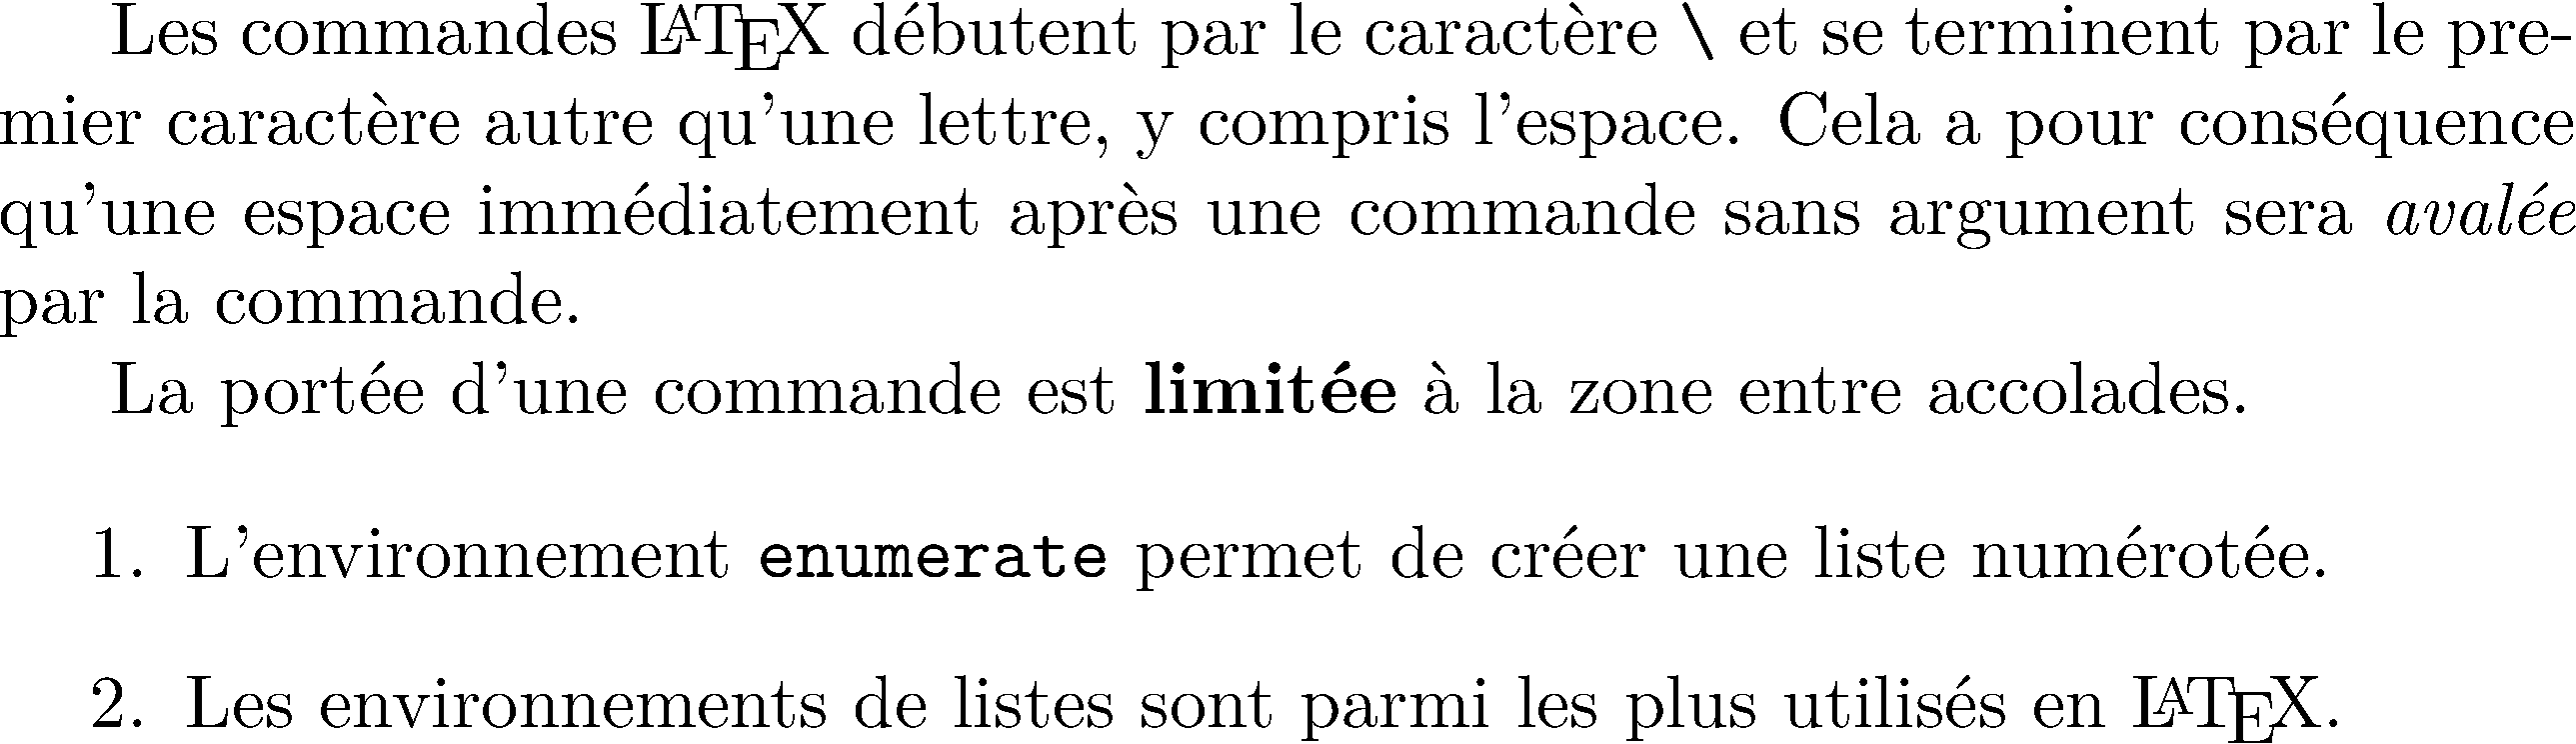
\includegraphics[width=0.95\linewidth]{exercice_commandes-output}}
  \end{center}
\end{frame}
%%% <<<

\subsection{Caractères spéciaux}

\begin{frame}[fragile=singleslide]
  \frametitle{Caractères spéciaux}
  \begin{itemize}
  \item Caractères réservés par {\TeX}:
    \begin{quote}
      \verb=# $ & ~ _ ^ % { }=
    \end{quote}
  \item Pour les utiliser, précéder par \verb=\=:
    \begin{demo}
      \begin{minipage}{0.15\linewidth}
        \begin{texample}
\begin{lstlisting}
\#
\end{lstlisting}
          \producing
          \#
        \end{texample}
      \end{minipage}
      \hfill
      \begin{minipage}{0.15\linewidth}
        \begin{texample}
\begin{lstlisting}
\$
\end{lstlisting}
          \producing
          \$
        \end{texample}
      \end{minipage}
      \hfill
      \begin{minipage}{0.15\linewidth}
        \begin{texample}
\begin{lstlisting}
\%
\end{lstlisting}
          \producing
          \%
        \end{texample}
      \end{minipage}
      \\
      \begin{minipage}{0.15\linewidth}
        \begin{texample}
\begin{lstlisting}
\_
\end{lstlisting}
          \producing
          \_
        \end{texample}
      \end{minipage}
      \hfill
      \begin{minipage}{0.15\linewidth}
        \begin{texample}
\begin{lstlisting}
\{
\end{lstlisting}
          \producing
          \}
        \end{texample}
      \end{minipage}
      \hfill
      \begin{minipage}{0.15\linewidth}
        \begin{texample}
\begin{lstlisting}
\}
\end{lstlisting}
          \producing
          \}
        \end{texample}
      \end{minipage}
    \end{demo}
  \item On écrira donc
    \begin{demo}
      \begin{texample}
\begin{lstlisting}
L'augmentation de 2~\$
représente une hausse
de 5~\%.
\end{lstlisting}
        \producing
        L'augmentation de 2~\$ représente une
        hausse de 5~\%.
      \end{texample}
    \end{demo}
  \end{itemize}
\end{frame}

\begin{frame}[fragile=singleslide]
  \frametitle{Caractères spéciaux (suite)}
  \begin{itemize}
  \item Espace insécable: \verb=~= %
\begin{lstlisting}
M.~Tremblay me doit 200~\$.
\end{lstlisting}
  \item Guillemets:
    \begin{demo}
      \begin{texample}
\begin{lstlisting}[escapeinside={}]
``guillemets anglais''
\end{lstlisting}
        \producing
        ``guillemets anglais''
      \end{texample}
      \begin{texample}
\begin{lstlisting}
«guillemets français»
\end{lstlisting}
        \producing
        «guillemets français»
      \end{texample}
   \end{demo}
  \item Tiret, tiret demi-cadratin, tiret cadratin:
    \begin{demo}
      \begin{minipage}{0.15\linewidth}
        \begin{texample}
\begin{lstlisting}
-
\end{lstlisting}
          \producing
          -
        \end{texample}
      \end{minipage}
      \hfill
      \begin{minipage}{0.15\linewidth}
        \begin{texample}
\begin{lstlisting}
--
\end{lstlisting}
          \producing
          --
        \end{texample}
      \end{minipage}
      \hfill
      \begin{minipage}{0.15\linewidth}
        \begin{texample}
\begin{lstlisting}
---
\end{lstlisting}
          \producing
          ---
        \end{texample}
      \end{minipage}
      \hfill
    \end{demo}
  \end{itemize}
\end{frame}

\begin{frame}[fragile]
  \frametitle{{\LaTeX} en français --- préambule pour pdf{\LaTeX}}

  Il faut charger un certain nombre de paquetages pour franciser \LaTeX.
\begin{lstlisting}
\documentclass[`\alt<2>{\textcolor{emphasis}{french}}{french}']{memoir}
  \usepackage{`\alt<2>{\textcolor{emphasis}{babel}}{babel}'}
  \usepackage[autolanguage]{`\alt<5>{\textcolor{emphasis}{numprint}}{numprint}'}
  \usepackage[utf8]{`\alt<3>{\textcolor{emphasis}{inputenc}}{inputenc}'}
  \usepackage[T1]{`\alt<3>{\textcolor{emphasis}{fontenc}}{fontenc}'}
  \usepackage{`\alt<4>{\textcolor{emphasis}{icomma}}{icomma}'}
\end{lstlisting}
  \pause
  \begin{itemize}[<+->]
  \item \pkg{babel}: traduction des mots-clés prédéfinis,
    typographie française, coupure de mots, document multilingue
  \item \pkg{inputenc} et \pkg{fontenc}: lettres accentuées dans le
    code source
  \item \pkg{icomma}: virgule comme séparateur décimal
  \item \pkg{numprint}: espace comme séparateur des milliers
  \end{itemize}
\end{frame}

\begin{frame}[fragile]
  \frametitle{{\LaTeX} en français --- préambule pour {\XeLaTeX}}

  {\XeLaTeX} supporte nativement les caractères UTF-8 dans le code source.
\begin{lstlisting}
\documentclass[french]{memoir}
  \usepackage{babel}
  \usepackage[autolanguage]{numprint}
  \usepackage{`\textcolor{emphasis}{fontspec}'}
  \usepackage{icomma}
\end{lstlisting}
  \begin{itemize}
  \item \pkg{fontspec}: gestion des polices et lettres accentuées dans
    le fichier PDF
  \end{itemize}
\end{frame}

%%% Local Variables:
%%% mode: latex
%%% TeX-engine: xetex
%%% TeX-master: "formation-latex-ul-diapos"
%%% End:
